\documentclass{article}

\usepackage{amsmath}
\usepackage[utf8]{inputenc}
\usepackage{amssymb}
\usepackage{amsxtra}
\usepackage{listings}
\usepackage{graphicx}
\usepackage[labelfont=bf]{caption}
\usepackage{cite}

% TODO
% - Add references
% - Replace repeated text like "This allows the network ..."
% - Shorten descriptions of figures
% https://www.scribbr.com/paraphrasing-tool/
% https://quillbot.com/?gspk=cmljaGFyZG1lZXV3c2VuNDkyMQ&gsxid=ZdcTN1uLPa5o&pscd=try.quillbot.com

\graphicspath{ {figures/} }

\newcommand{\refchapter}[1]{Chapter~\ref{#1}}
\newcommand{\refsec}[1]{Section~\ref{#1}}
\newcommand{\refeqn}[1]{Equation~(\ref{#1})}
\newcommand{\reffig}[1]{Figure~\ref{#1}}

\title{
  {\bf \scriptsize
    RHEINISCH-WESTF\"ALISCHE TECHNISCHE HOCHSCHULE AACHEN \\
    Neuroinspired Computing (Prof. Dr. Abigail Morrison)
  } \vspace{2cm} \\
  Deterministic Recurrent Neural Networks \\
  {\large Seminar Thesis} 
}
\author{Marco Bischoff (Matr.-Nr. 370222)}

\begin{document}


\pagestyle{headings}

\maketitle
\newpage

\tableofcontents
\newpage



\section{Introduction}
\label{ch:1}

Machine learning has seen a rapid evolution in recent years, with neural networks emerging
as a powerful tool for a wide range of applications. Initially inspired by the structure
and function of the human brain, artificial neural networks have evolved into a diverse
family of models, each tailored to specific tasks and data types. In particular, Recurrent
Neural Networks (RNNs) have revolutionized the processing of sequential data, enabling
tasks such as language modeling \cite{merity2017regularizing}, machine translation
\cite{choLearningPhraseRepresentations2014}, and speech recognition
\cite{graves2013speech}. In this paper, we explore the architecture and operation of RNNs,
with a focus on Long Short-Term Memory (LSTM) networks, which are designed to learn
long-term dependencies more effectively than standard RNNs. We also discuss the Neural
Turing Machine (NTM), which is a type of recurrent neural network that is augmented with
an external memory bank.


\subsection{Feedforward Neural Networks}
\label{sec:1.0}

Before delving into the realm of RNNs, it is essential to understand the foundational
concepts of feedforward neural networks, which form the basis for more complex models such
as RNNs. Feedforward neural networks, also known as multilayer perceptrons, are a class of
neural networks that process input data through a series of interconnected layers. Each
layer consists of a set of nodes, or neurons, which perform a weighted sum of the inputs
followed by the application of an activation function. The output of each layer serves as
the input to the next layer, ultimately producing a final output. The process of training
a feedforward neural network involves adjusting the weights of the connections between
neurons to minimize the difference between the predicted and actual outputs, typically
using the backpropagation algorithm and gradient descent \cite{mitchell_machine_1997}.

This poses a limitation on the types of data that can be processed by feedforward neural
networks, as they are designed to operate on fixed-size input vectors and produce
fixed-size output vectors. This constraint makes them ill-suited for tasks involving
sequential data, where the length of the input and output sequences may vary. For example,
in natural language processing, the length of a sentence can vary significantly, making it
challenging to process using a feedforward neural network \cite{Sundermeyer2015}.
Additionally, feedforward neural networks lack an internal state, meaning they do not have
the ability to remember information from previous inputs. This makes it difficult for them
to capture the sequential dependencies present in many real-world datasets. To address
these limitations, we turn to Recurrent Neural Networks.



\section{Recurrent Neural Networks}
\label{ch:2}

Recurrent Neural Networks (RNNs) are a class of neural networks that are designed to
handle sequential data by maintaining an internal state. Unlike feedforward neural
networks, which process the entire input at once, RNNs process the input elements
one at a time, allowing them to capture dependencies over time.

\begin{figure}[htbp]
  \centering
  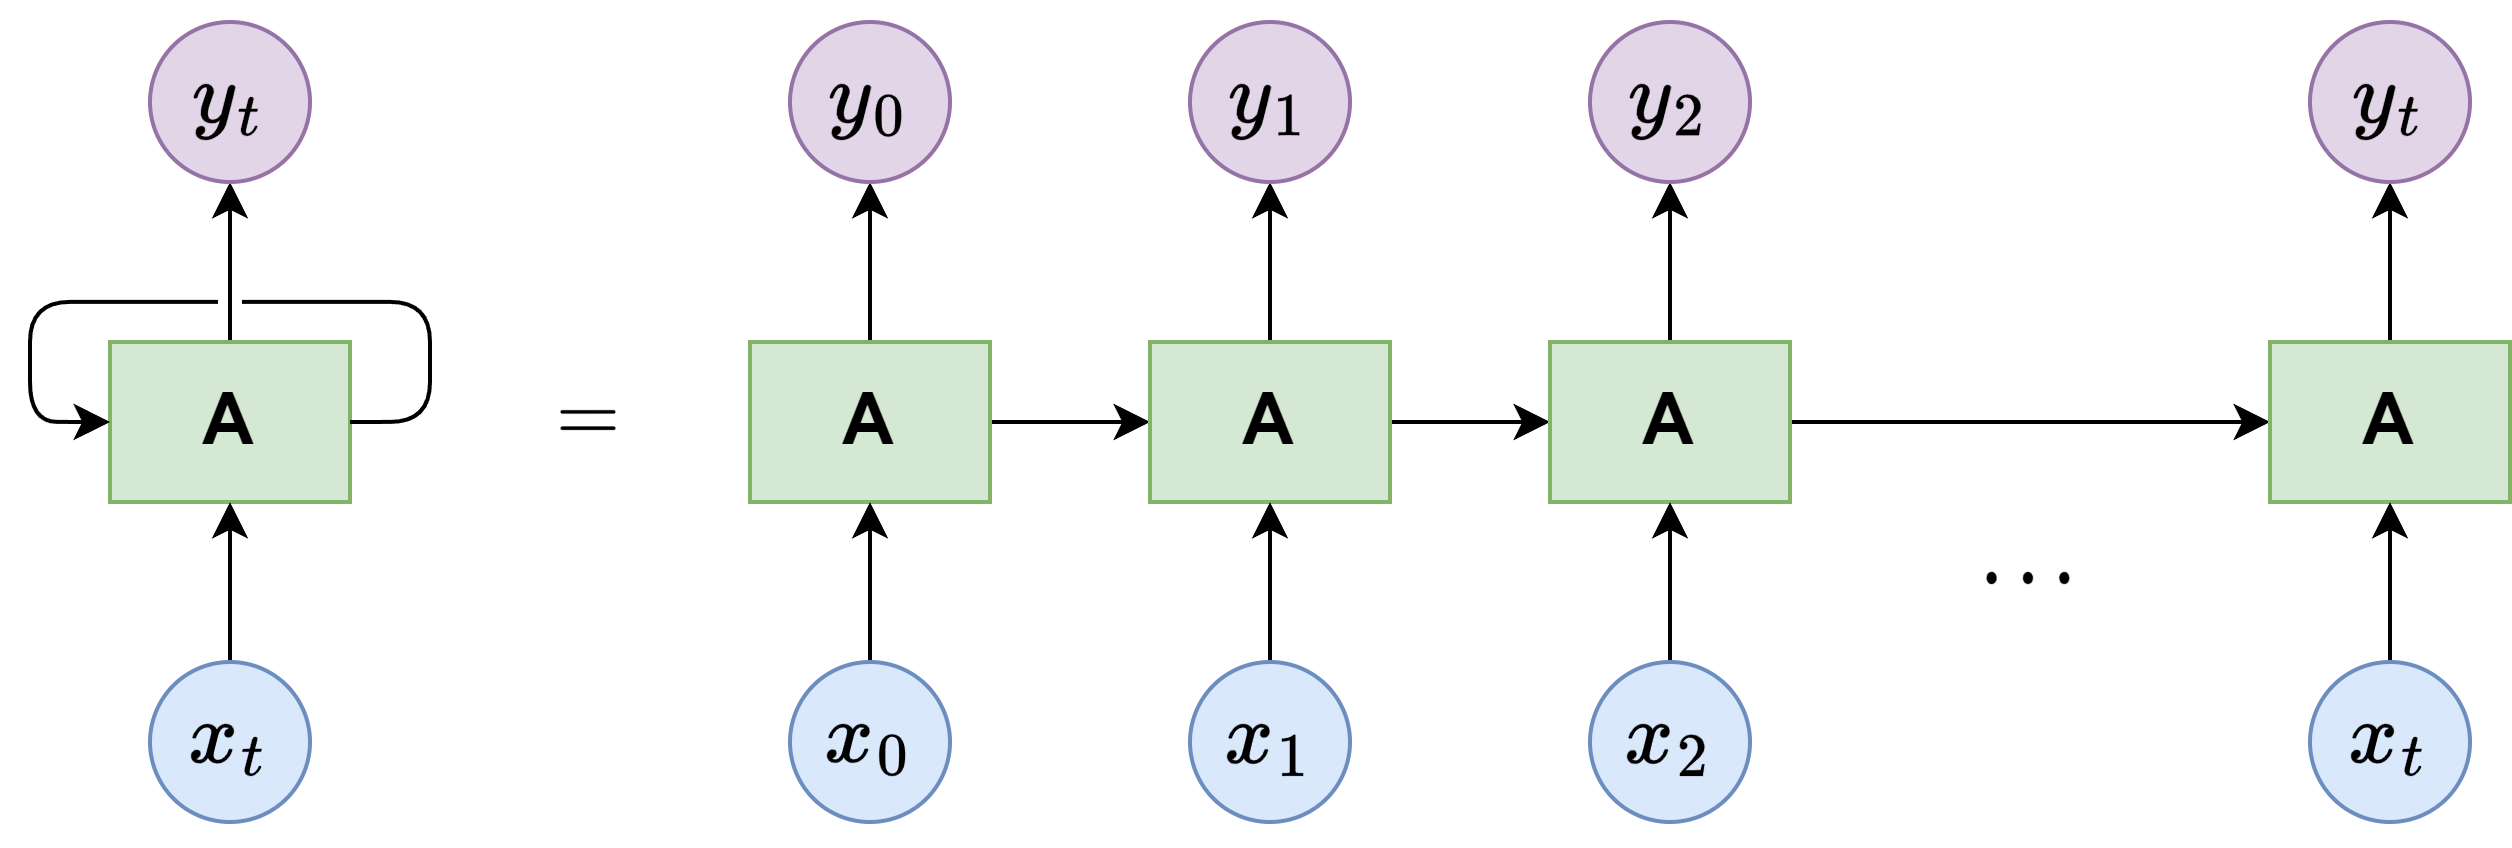
\includegraphics[width=0.9\textwidth]{RNN Unrolled.drawio.png}
  \caption{A recurrent neural network unrolled into a sequence of layers. The input
    sequence $x_0, x_1, \ldots, x_t$ is shown in blue, the network layer in green and the
    output sequence $y_0, y_1, \ldots, y_t$ in purple.}
  \label{fig:rnn-unrolled}
\end{figure}

In its simplest form, the structure of an RNN is the same as a feedforward neural network,
with the addition of a feedback loop to maintain an internal state, which is updated at
each time step, allowing the network to remember information from previous inputs. The
output of the network at each time step is influenced not only by the current input but
also by the internal state. This means that, instead of having multiple layers with
separate weights, RNNs have a single layer that acts as a dynamical system, changing over
time. The repeating module in an RNN can be unrolled into a sequence of interconnected
layers, allowing the network to process sequences of arbitrary length, as shown in
\reffig{fig:rnn-unrolled}. This unrolling reveals that RNNs are intimately related to
sequences and lists, making them a natural architecture for processing data of this form.

\subsection{Categories of Applications}
\label{sec:2.0}

\begin{figure}[htbp]
  \centering
  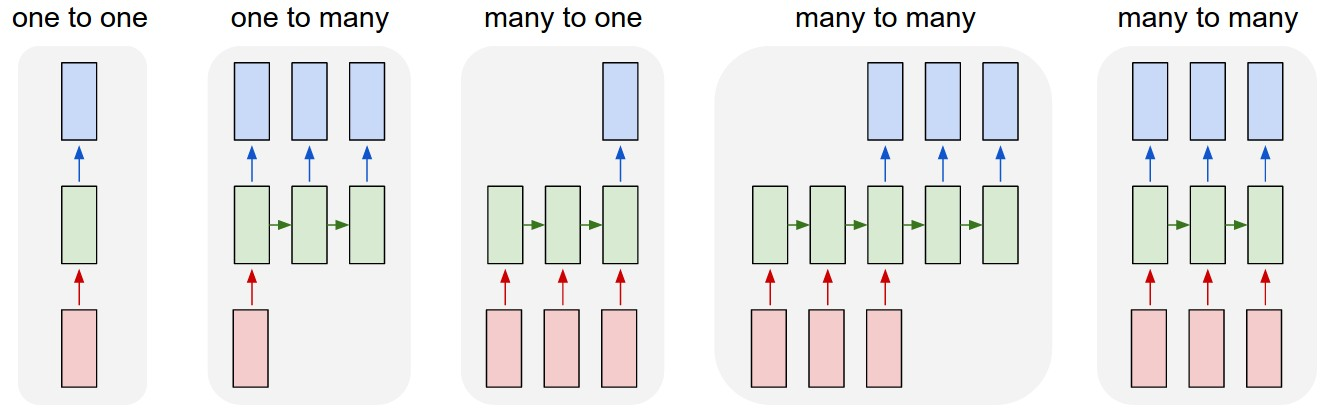
\includegraphics[width=0.9\textwidth]{Karpathy application types.jpeg}
  \caption{Ways of applying RNNs to different types of data. Both the input and output can
    be a fixed-size vector or a sequence of vectors. If both are sequences, the input and
    output vectors can either be regarded as pairs or as unrelated sequences of different
    lengths. \cite{karpathyUnreasonableEffectivenessRecurrent}}
  \label{fig:rnn-application-types}
\end{figure}

The applications of RNNs can be categorized based on the length of the input and output
sequences and the relationship between them, as shown in
\reffig{fig:rnn-application-types}. For example, for tasks such as image classification,
where the input and output sequences are of fixed length, RNNs can be used in a manner
similar to feedforward neural networks (one-to-one). They can also be used for tasks such
as image captioning, where the input is a fixed-size image and the output is a sequence of
words (one-to-many). Additionally, RNNs can be used for tasks such as sentiment analysis,
where the input is a sequence of words and the output is a single value (many-to-one).
Tasks, where both the input and output are sequences of varying lengths (many-to-many),
can be categorized into two subtypes. For example, in machine translation, the input
sequence is processed first, and then the output sequence is generated. In contrast, for
video classification, the output is generated simultaneously with the input, allowing the
network to use the previous frames as context. This demonstrates the flexibility of RNNs
in handling a wide range of tasks involving sequential data.

% Possible extensions: Sequential processing in absence of sequences


\subsection{Internal Structure}
\label{sec:2.1}

\begin{figure}[htbp]
  \centering
  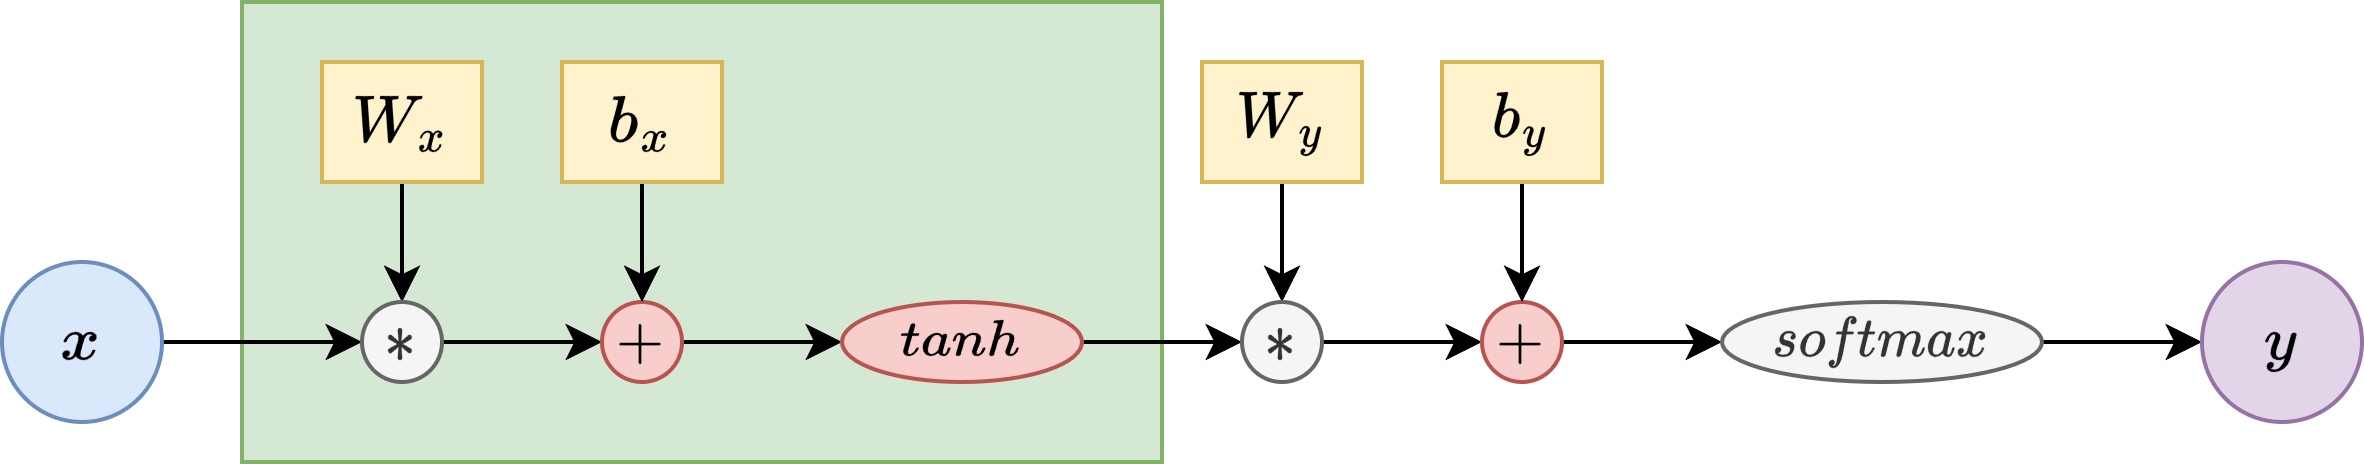
\includegraphics[width=0.9\textwidth]{Block Diagram Feedforward.drawio.png}
  \caption{The internal structure of a feedforward neural network with a single layer. The
    input vector $x$ is transformed by a linear transformation $Wx + b$ and then passed
    through an activation function. The output can, for example, be processed with another
    linear transformation and a softmax function to produce a probability distribution
    over classes. The vector $y$ is the output of the network. In a multi-layer network,
    the components in the green box would be repeated for each layer.}
  \label{fig:internal-feedforward}
\end{figure}

\begin{figure}[htbp]
  \centering
  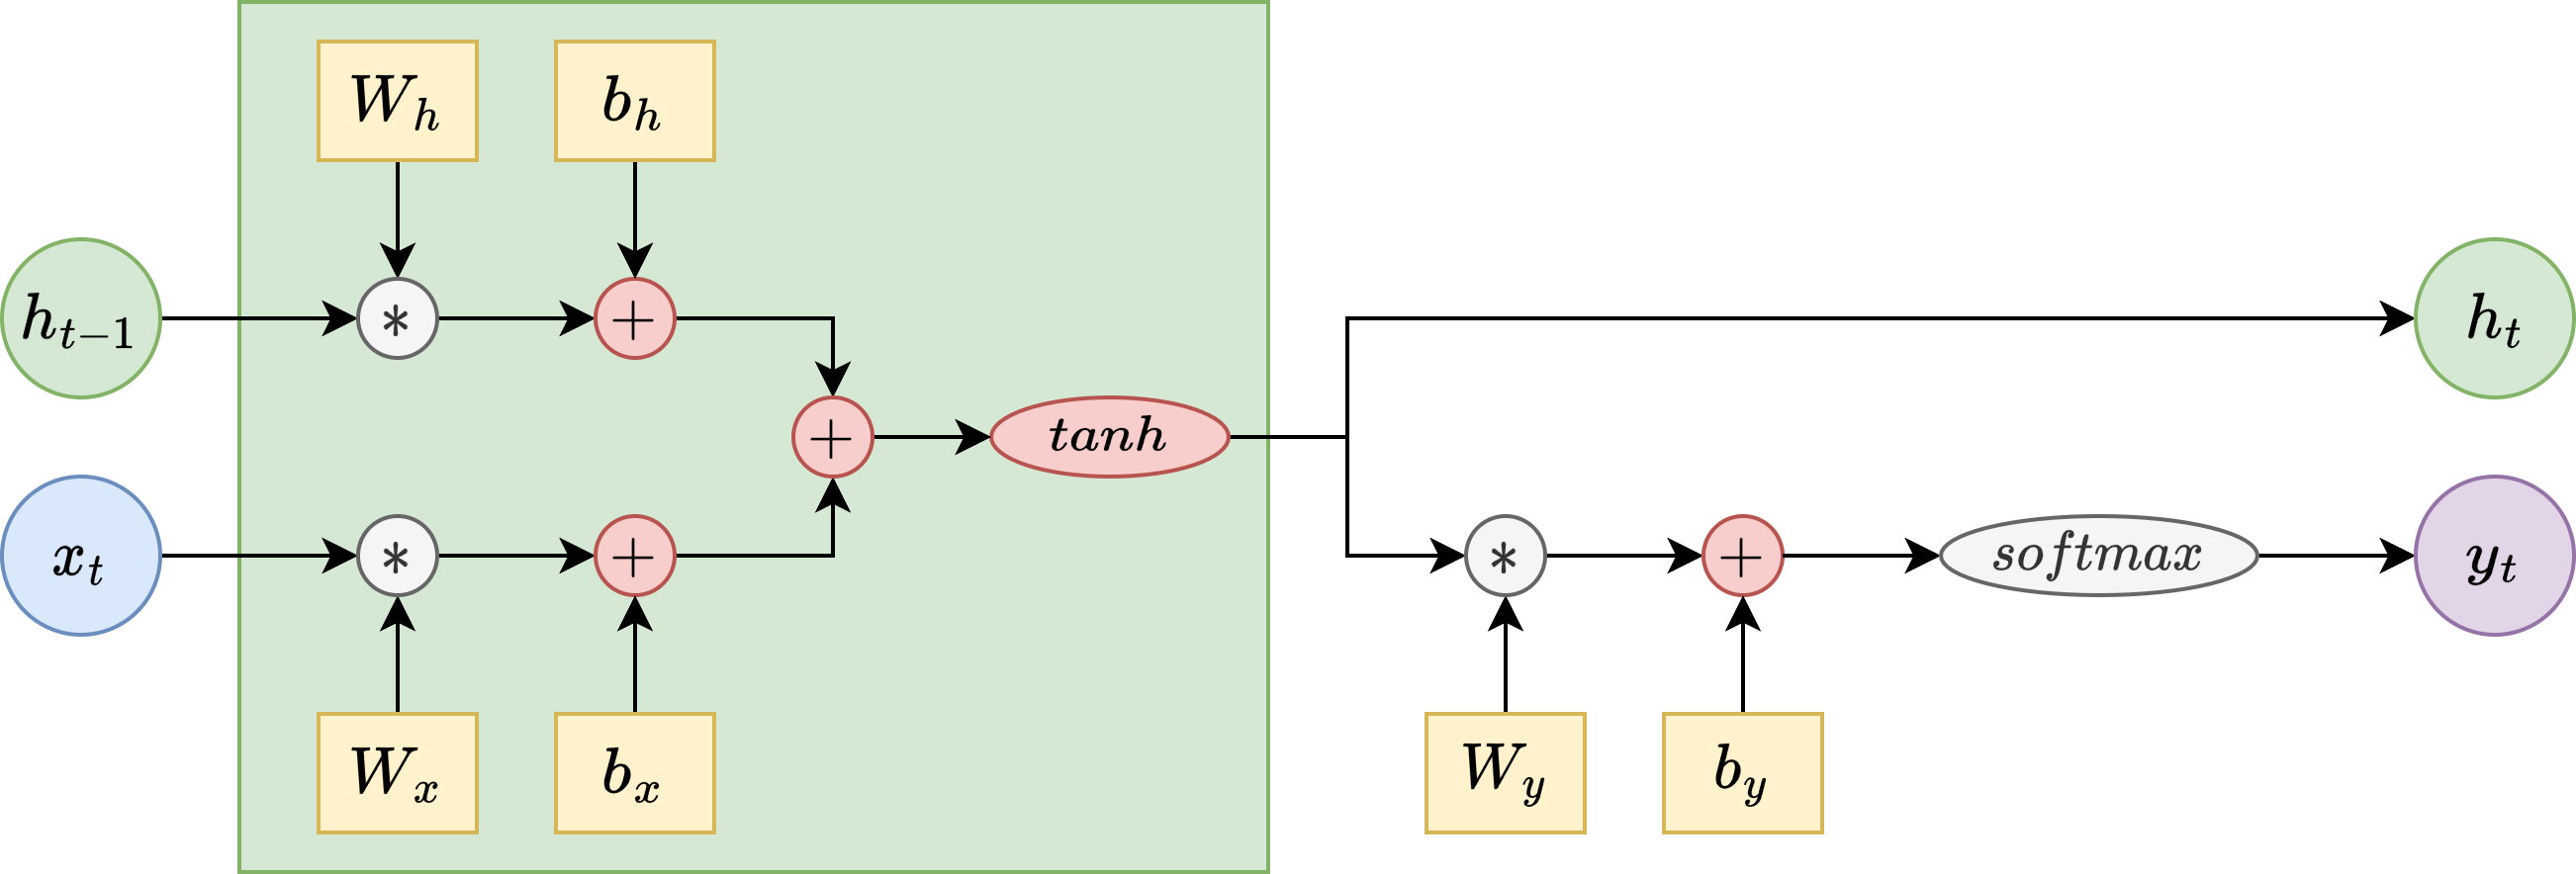
\includegraphics[width=0.9\textwidth]{Block Diagram RNN.drawio.png}
  \caption{The internal structure of a recurrent neural network with a single layer. The
    input vector $x$ and the previous state vector $h_{t-1}$ are concatenated and
    transformed by a linear transformation and an activation function to produce the new
    state vector $h_t$. To produce the output vector $y_t$, the state vector can, for
    example, be transformed by another linear transformation and a softmax function.}
  \label{fig:internal-rnn}
\end{figure}

To understand the internal structure of an RNN, we compare a single layer feedforward NN
with a single layer RNN. As shown in \reffig{fig:internal-feedforward}, a feedforward NN
transforms the input vector $x$ by a linear transformation and an activation function to
produce the output of a single layer. In contrast, as shown in \reffig{fig:internal-rnn},
an RNN first concatenates the input vector $x$ with the previous state vector $h_{t-1}$,
then transforms the concatenated vector in the same way as a feedforward NN. The resulting
state vector $h_t$ then serves as the input to the next time step. For the first iteration
of the RNN, the previous state vector is typically initialized to a vector of zeros.
However, it can also be learned as part of the training process, which can boost the
performance of the network in some cases
\cite{sutskeverImportanceInitializationMomentum2013}.


\subsection{Backpropagation}
\label{sec:2.2}

% First, introduce regular backpropagation
The training of RNNs is typically performed using the backpropagation through time (BPTT)
algorithm, which is an extension of the backpropagation algorithm used to train
feedforward neural networks. As an example, consider a single layer feedforward NN, like
the green box in \reffig{fig:internal-feedforward}. Let
\begin{itemize}
  \item $x$ be the input vector,
  \item $W$ the weight matrix,
  \item $b$ the bias vector,
  \item $y$ the output vector,
  \item $t$ the target vector (ground truth)
  \item $\sigma$ the activation function, and
  \item $L = \frac{1}{2} \sum_{i=1}^{n} (t_i - y_i)^2$ the loss function (e.g. mean
        squared error).
\end{itemize}
We first do a forward pass to compute the output $y = \sigma(Wx + b)$ and compare it to
the target $t$ by the loss function $L$. Then, we do a backward pass to compute the
gradient of the loss function with respect to the weights and biases of the network. Here,
we use the chain rule of calculus:
\begin{align}
  \frac{\partial L}{\partial W} & = \frac{\partial L}{\partial y} \frac{\partial y}{\partial W}                                             \\
                                & = \frac{\partial L}{\partial y} \frac{\partial y}{\partial (Wx + b)} \frac{\partial (Wx + b)}{\partial W} \\
                                & = -(t-y) \cdot \sigma'(Wx + b) \cdot x^T
\end{align}
The gradient for the bias vector $\frac{\partial L}{\partial b}$ can be computed
similarly. For a network with multiple layers, the gradients are computed layer by layer
using the chain rule, starting from the output layer and moving backwards through the
network. In the final step, the weights and biases are updated in the direction that
minimizes the loss: $W \leftarrow W - \alpha \frac{\partial L}{\partial W}$ and $b
  \leftarrow b - \alpha \frac{\partial L}{\partial b}$, where $\alpha$ is the learning rate.
This is usually done using an optimization algorithm such as stochastic gradient descent.

% Then, explain how BPTT differs
The BPTT algorithm extends this approach to RNNs by unrolling the network into a sequence
of interconnected layers, as shown in \reffig{fig:rnn-unrolled}. The forward pass is
performed as usual, with the output of each time step serving as the input to the next
time step. The backward pass then accumulates the gradients over the entire sequence and
updates the weights and biases accordingly. This allows the network to capture the
dependencies between the input elements and learn from the entire sequence, rather than
just the current input. The key difference between BPTT and regular backpropagation is
that the weights of the RNN are shared across time steps, meaning that the same weights
are used at each time step. Also, the number of time steps is not given by the number of
layers, but by the length of the input sequence. For long sequences, this can lead to
problems such as vanishing or exploding gradients, which can make training difficult.


\subsection{The Problem of Long-Term Dependencies}
\label{sec:2.3}

One of the key challenges in training RNNs is the problem of long-term dependencies. To
illustrate this, consider a simplified RNN \cite{pascanuDifficultyTrainingRecurrent2013}
that takes an input sequence $x_0, x_1, \ldots, x_n$ and produces a sequence of
outputs/hidden states $h_0, h_1, \ldots, h_n$. It is defined by the function $F$ for each
time step $t \in \{0, 1, \ldots, n\}$:
\begin{equation}
  h_t = F(h_{t-1}, x_t) = W_h \tanh{h_{t-1}} + W_x x_t + b
\end{equation}
Then the gradient with respect to the hidden state at time step $t$ is given by:
\begin{equation}
  \label{eq:gradient-hidden-state}
  \nabla_h F(h_{t-1}, x_t) = W_h \text{diag}(\tanh'(h_{t-1}))
\end{equation}
For the backward pass, we need to compute the gradient of the loss function, which in
this case is given by
\begin{equation}
  \partial L = \nabla_h L(h_n, x_1, \ldots, x_n) \cdot \sum_{t=1}^{n} \prod_{k=n-t+1}^{n} \nabla_h F(h_{k-1}, x_k)
\end{equation}
where each term in the sum is the gradient of the current layer. The sum can be written
as:
\begin{align}
   & \sum_{t=1}^{n} \prod_{k=n-t+1}^{n} \nabla_h F(h_{k-1}, x_k)                                      \label{eq:gradient-sum} \\
   & = \nabla_h F(h_{n-1}, x_n)                                                                       \nonumber               \\
   & + \nabla_h F(h_{n-1}, x_n) \cdot \nabla_h F(h_{n-2}, x_{n-1})                                    \nonumber               \\
   & + \nabla_h F(h_{n-1}, x_n) \cdot \nabla_h F(h_{n-2}, x_{n-1}) \cdot \nabla_h F(h_{n-3}, x_{n-2}) \nonumber               \\
   & + \ldots \nonumber
\end{align}
With \refeqn{eq:gradient-hidden-state} and \refeqn{eq:gradient-sum}, we can see that the
gradient for time step $t$ is predominantly influenced by $W_h^{n-t+1}$. If the largest
singular value of $W_h$ is less than 1, the gradient will vanish as $t$ increases. If it
is greater than 1, the gradient will explode
\cite{pascanuDifficultyTrainingRecurrent2013}. This makes it difficult for the network to
learn long-term dependencies, as the gradients become too small or too large to be useful.
This is known as the problem of long-term dependencies, and it is a fundamental limitation
of standard RNNs.

Multiple approaches have been proposed to address this problem, for example, clipping the
gradient to prevent it from becoming too large
\cite{pascanuDifficultyTrainingRecurrent2013}. Let $\nabla_W L$ be the gradient of the
loss function and $\epsilon$ a small constant. Then the clipped gradient $\nabla$ is
\begin{equation}
  \nabla =
  \begin{cases}
    \nabla_W L                                       & \text{if } ||\nabla_W L|| < \epsilon \\
    \epsilon \cdot \frac{\nabla_W L}{||\nabla_W L||} & \text{otherwise}
  \end{cases}
\end{equation}
This prevents the gradient from becoming too large, but it does not address the problem of
vanishing gradients. Another approach is to use ReLU activation functions
\cite{glorotDeepSparseRectifier2010}, which have the advantage of not saturating for
positive inputs because their derivative is 1. However, the problem of vanishing gradients
still remains for negative inputs. Moreover, there were methods proposed to initialize the
weights of the network in a way that prevents the gradients from vanishing or exploding
\cite{kumar2017weight}. While these methods can mitigate the problem of long-term
dependencies to some extent, they do not provide a complete solution. A more effective
approach is to use Long Short-Term Memory (LSTM) networks, which were specifically
developed to address the problem of vanishing and exploding gradients in RNNs.



\section{Long Short-Term Memory Networks}
\label{ch:3}

Long Short-Term Memory (LSTM) networks are a special type of RNN that are designed to
learn long-term dependencies more effectively than standard RNNs. They were introduced by
Hochreiter and Schmidhuber in 1997 \cite{hochreiterLongShorttermMemory1997} and have since
become a popular choice for a wide range of applications, including language generation,
medical diagnosis, sentiment analysis and video processing. The key idea behind LSTMs is
the use of a memory cell, which allows the network to store and access information over
long time scales. In this section, we explore the architecture and operation of LSTMs, as
well as their applications and variants.


\subsection{Architecture}
\label{sec:3.0}

\begin{figure}
  \centering
  \includegraphics[width=0.9\textwidth]{LSTM Architecture.drawio.png}
  \caption{The repeating module of an LSTM network. Each yellow box represents a neural
    network layer with its activation function and the pink circles represent pointwise
    operations. The lines merging denote concatenation, while a line forking denotes its
    content being copied. The output is denoted by $h_t$. \cite{olahUnderstandingLSTM}}
  \label{fig:lstm}
\end{figure}

The architecture of an LSTM network is based on a repeating module that contains four
interacting layers, as shown in \reffig{fig:lstm}. The key to LSTMs is the cell state
$C_t$, which runs straight down the entire chain with only minor linear interactions. This
allows information to flow along the cell state unchanged, making it easy for the network
to remember information over long time scales. The cell state is regulated by structures
called gates, which are composed of neural network layers and pointwise operations. The
gates allow the network to control the flow of information into and out of the cell state,
enabling it to remember or forget information as needed.


\subsubsection{Forget Gate}
\label{sec:3.0.0}

The first step in the operation of an LSTM is to decide what information to forget from
the cell state. This is done by a sigmoid layer called the forget gate layer, which takes
the previous hidden state $h_{t-1}$ and the current input $x_t$ as input and outputs a
number between $0$ and $1$ for each element in the cell state $C_{t-1}$. A value of $0$
indicates that the corresponding element should be forgotten, while a value of $1$
indicates that it should be retained. This allows the network to selectively forget
information from the cell state as needed, enabling it to discard irrelevant information
and focus on the most important elements.
\begin{equation}
  f_t = \sigma(W_f \cdot [h_{t-1}, x_t] + b_f)
\end{equation}


\subsubsection{Input Gate}
\label{sec:3.0.1}

The next step is to decide what new information to store in the cell state. This has two
parts. First, a sigmoid layer called the input gate layer decides which values to update.
Next, a tanh layer creates a vector of new candidate values $\tilde{C}_t$ that could be
added to the state. The input gate layer outputs a number between $0$ and $1$ for each
element in the cell state, indicating how much of the new candidate values should be added
to the state. This allows the network to selectively update the cell state with new
information, enabling it to incorporate relevant information from the current input.
\begin{align}
  i_t         & = \sigma(W_i \cdot [h_{t-1}, x_t] + b_i) \\
  \tilde{C}_t & = \tanh(W_C \cdot [h_{t-1}, x_t] + b_C)
\end{align}


\subsubsection{Update Cell State}
\label{sec:3.0.2}

The next step is to update the old cell state $C_{t-1}$ into the new cell state $C_t$. The
previous steps have already decided what to do, so the network just needs to actually do
it. First, the old state is multiplied by the forget gate $f_t$, forgetting the things
that were decided to forget earlier. Then, the new candidate values $\tilde{C}_t$ are added
to the state, scaled by how much the input gate decided to update each state value.
\begin{equation}
  C_t = f_t \cdot C_{t-1} + i_t \cdot \tilde{C}_t
\end{equation}


\subsubsection{Output Gate}
\label{sec:3.0.3}

Finally, the network needs to decide what to output. This output will be based on the cell
state, but will be a filtered version. First, a sigmoid layer called the output gate layer
decides what parts of the cell state should be output. Then, the cell state is put through
a tanh function to push the values to be between $-1$ and $1$, and multiplied by the
output of the sigmoid gate. The result is the output of the network at the current time
step $h_t$, which can be used for further processing or as the final output of the
network.
\begin{align}
  o_t & = \sigma(W_o \cdot [h_{t-1}, x_t] + b_o) \\
  h_t & = o_t \cdot \tanh(C_t)
\end{align}


\subsection{Variants}
\label{sec:3.1}

LSTMs have been the subject of extensive research, leading to the development of several
variants that aim to improve their performance and address specific challenges
\cite{greffLSTMSearchSpace2017}. One popular variant, introduced by Gers and Schmidhuber
in 2000 \cite{gersRecurrentNetsTime2000}, adds peephole connections to the architecture
of the LSTM. These connections allow the cell to control the gates more precisely, making
it easier for the network to learn precise timings. Additionally, the output activation
function is omitted, as there is no evidence that it is essential for solving the problems
that LSTMs have been tested on so far.

% Variant: Dynamic Cortex Memory
% TODO: This is copy paste from the abstract
Another variant, called Dynamic Cortex Memory (DCM), was introduced by Otte et al. in 2014
\cite{otte2014dynamic}. The DCM is an extension of the LSTM model that enhances the inner
interplay of the gates and the error carousel due to several new and trainable
connections. These connections enable a direct signal transfer from the gates to one
another, allowing the network to converge faster during training with backpropagation
through time (BPTT) than LSTM under the same training conditions. Furthermore, DCMs yield
better generalization results than LSTMs, as shown for different supervised problem
scenarios, including storing precise values, adding, and learning a context-sensitive
grammar.

% Variant: Gated Recurrent Unit

\begin{figure}[htbp]
  \centering
  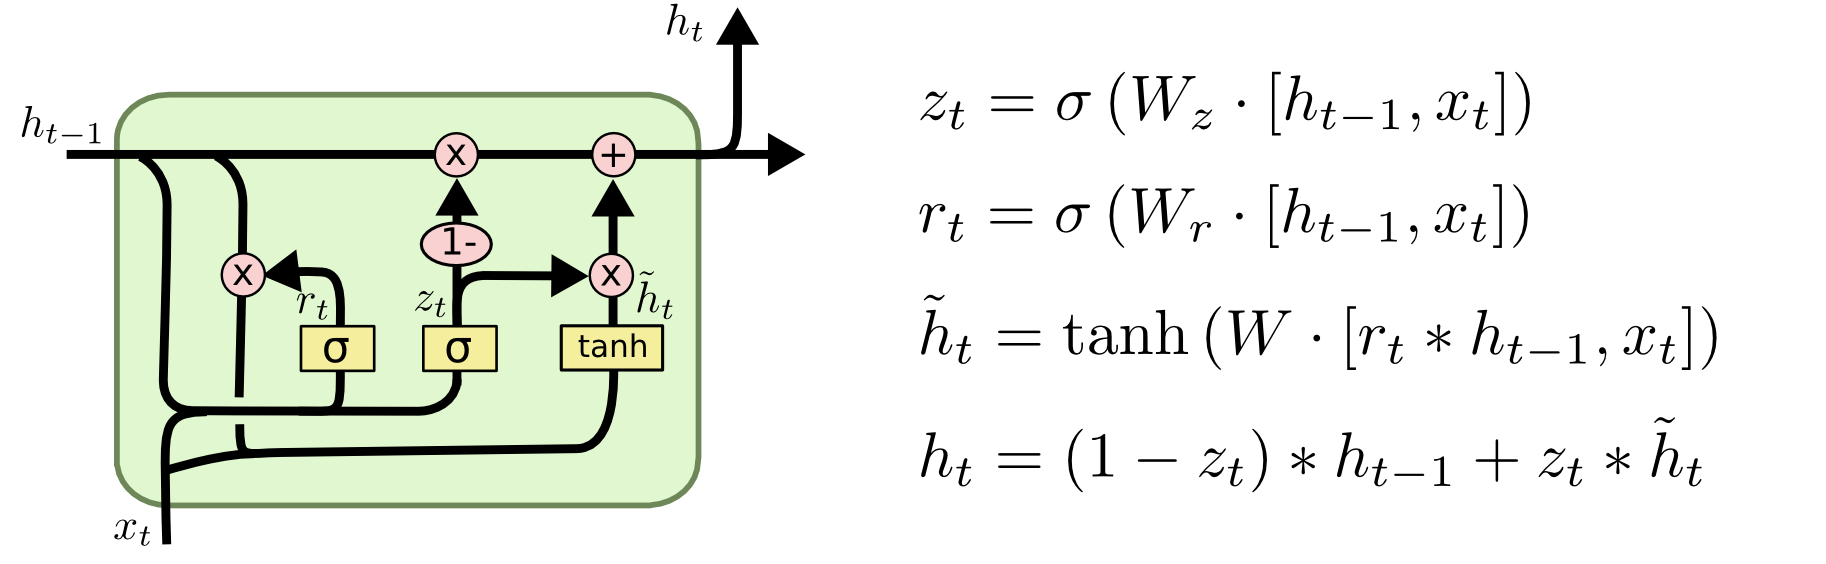
\includegraphics[width=0.9\textwidth]{LSTM3-var-GRU.png}
  \caption{The structure of a Gated Recurrent Unit (GRU) network. \cite{olahUnderstandingLSTM}}
  \label{fig:gru}
\end{figure}
One of the most well-known variants of the LSTM architecture is the Gated Recurrent Unit
(GRU), which was proposed by Cho et al. in 2014
\cite{choLearningPhraseRepresentations2014}. The GRU simplifies the LSTM architecture by
removing the output gate and the cell state, and combining the input and forget gates into
a single update gate. This reduces the number of parameters in the network and makes it
easier to train. The internal structure of a GRU network is shown in \reffig{fig:gru}.
While the GRU has been shown to perform comparably to the LSTM on many tasks, it has the
advantage of being simpler and more efficient, making it a popular choice for many
applications.



\section{Neural Turing Machines}
\label{ch:4}

% Maybe add: The algorithm combines both content-based addressing and location-based addressing

While LSTMs and their variants have proven to be effective for a wide range of tasks, they
are still limited in their ability to perform complex operations that require explicit
memory access. To address this limitation, Graves et al. introduced the Neural Turing
Machine (NTM) in 2014 \cite{gravesNeuralTuringMachines2014}. The NTM is a type of
recurrent neural network that is augmented with an external memory bank, allowing it to
perform complex operations that require explicit memory access.

The idea behind the NTM is to combine the power of neural networks with the ability to
store and retrieve information from an external memory bank. The approach is inspired by
the structure and operation of a Turing machine, which is a theoretical model of a
computer that can read from and write to an infinite tape of memory. A computer program
makes use of three fundamental mechanisms: elementary operations (e.g., arithmetic
operations), logical flow control (branching), and external memory, which can be written
to and read from in the course of computation \cite{von_neumann_first_1945}. In human
cognition, the process that shares the most similarity to algorithmic operation is known
as working memory, which is understood to mean a capacity for short-term storage of
information and its rule-based manipulation \cite{baddeley_memory_2009}.



\subsection{Architecture}
\label{sec:4.0}

\begin{figure}[htbp]
  \centering
  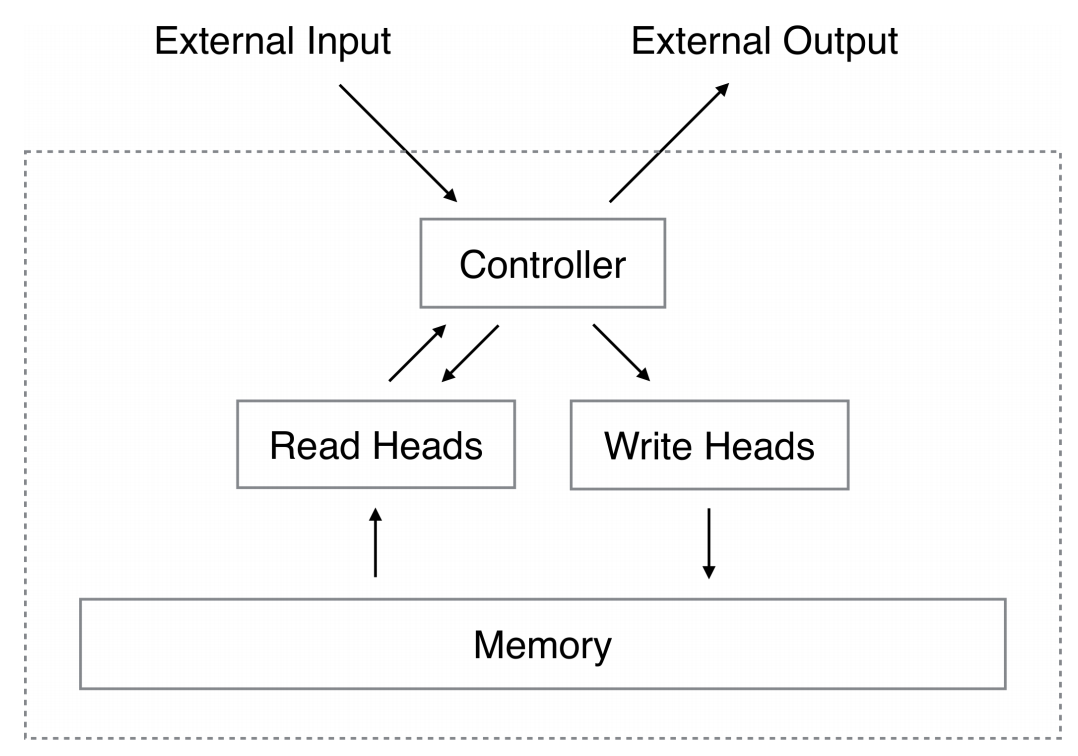
\includegraphics[width=0.7\textwidth]{NTM Structure.png}
  \caption{The architecture of a Neural Turing Machine.}
  \label{fig:ntm-structure}
\end{figure}

The architecture of an NTM is shown in \reffig{fig:ntm-structure}. The NTM consists of two
main components: a controller and a memory bank. The controller is an LSTM, which is
responsible for processing the input data and interacting with the memory bank. The memory
bank for time step $t$ is a matrix $\textbf{M}_t$ of size $N \times M$, where $N$ is the
number of memory locations and $M$ is the size of each memory location. The memory bank
can be read from and written to by the controller, allowing the network to store and
retrieve information as needed.

A key aspect of the NTM is that each operation of the NTM is differentiable, meaning that
it can be trained using backpropagation like a standard neural network. The controller
interacts with the memory bank using two main mechanisms: read heads and write heads,
which are responsible for reading and writing information from and to the memory bank,
respectively. The read and write heads use an attention mechanism to select the memory
locations to read from and write to, allowing the network to focus on the most relevant
information.


\subsection{Addressing Mechanism}
\label{sec:4.1}

\begin{figure}[htbp]
  \centering
  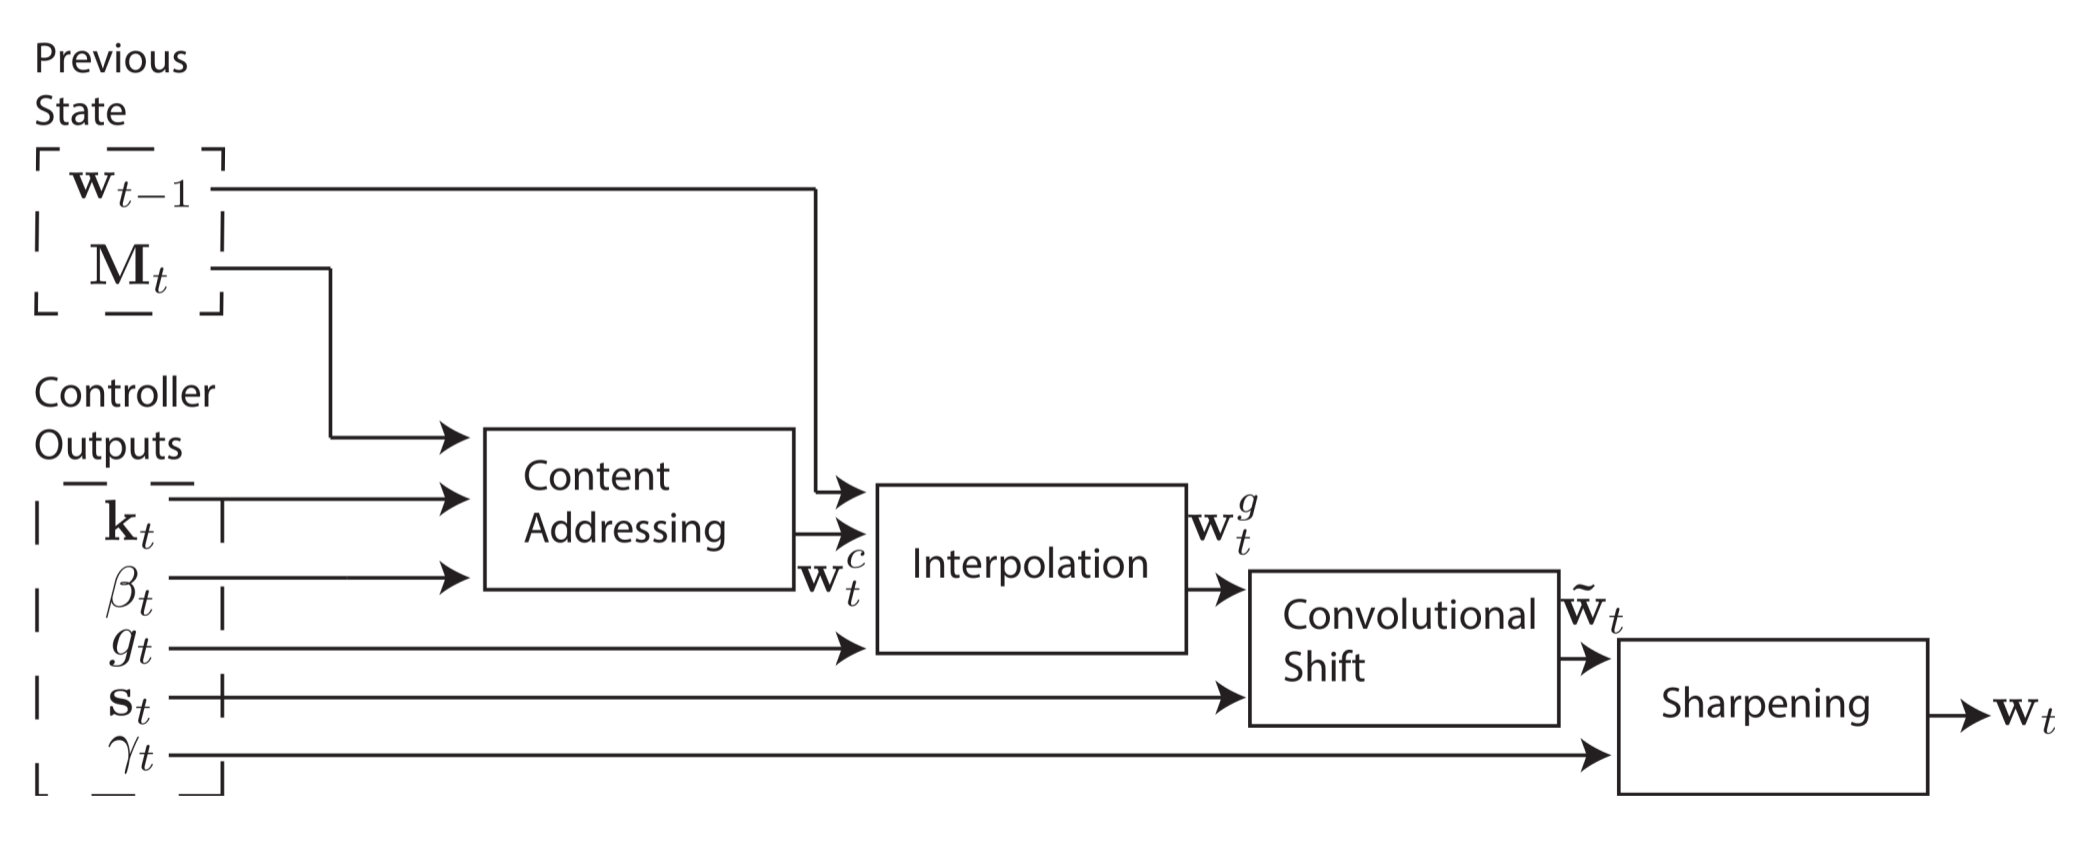
\includegraphics[width=0.9\textwidth]{ntm_addr_4.png}
  \caption{Flow diagram of the addressing mechanism in a Neural Turing Machine.
    \cite{gravesNeuralTuringMachines2014}}
  \label{fig:ntm-addressing}
\end{figure}

The addressing mechanism of an NTM is responsible for selecting the memory locations to
read from and write to. It consists of four main steps: content addressing, interpolation,
convolutional shift, and sharpening, as shown in \reffig{fig:ntm-addressing}. The
addressing mechanism is performed at each time step, allowing the controller to interact
with the memory bank in a dynamic and flexible manner.


\subsubsection{Content Addressing}
\label{sec:4.1.0}

The first step of the addressing mechanism is content addressing, which is responsible for
selecting the memory locations to read from and write to based on the content of the
memory. It takes the current memory bank $\textbf{M}_t$, the key vector $\textbf{k}_t$,
and the key strength $\beta_t$ as input. The key vector is used to calculate the
similarity between the key and each memory location using the cosine similarity measure
$K[\cdot, \cdot]$. The parameter $\beta_t$ amplifies the precision of the attention
weights, enforcing high sparsity in the weights.
\begin{equation}
  \textbf{w}_t^c = \text{softmax}(\beta_t K[\textbf{M}_t, \textbf{k}_t])
\end{equation}


\subsubsection{Interpolation}
\label{sec:4.1.1}

The next step is interpolation, which allows the network to iteratively access subsequent
memory locations. It takes the previous attention weights $\textbf{w}_{t-1}$, the content-based
attention weights $\textbf{w}_t^c$, and the interpolation gate $g_t \in (0, 1)$ as input. For a
value of $g_t = 0$, the previous attention weights are retained, while for a value of
$g_t = 1$, the current attention weights are used. This allows the network to blend
between the previous and current attention weights based on the value of $g_t$.
\begin{equation}
  \textbf{w}_t^g = g_t \textbf{w}_t^c + (1 - g_t) \textbf{w}_{t-1}
\end{equation}


\subsubsection{Convolutional Shift}
\label{sec:4.1.2}

After interpolation, each head produces a shift weighting $\textbf{s}_t$ that is used as
the kernel for a convolutional shift operation. This operation convolves the new attention
weights with the kernel $\textbf{s}_t$, allowing the network to shift the attention if
needed. This is useful for accessing memory locations in a flexible and dynamic manner.
All indices are modulo $N$ to ensure that the shift operation is circular.
\begin{equation}
  \tilde{\textbf{w}}_t(i) \leftarrow \sum_{j=0}^{N-1} \textbf{w}_t^g(j) \textbf{s}_t(i-j)
\end{equation}


\subsubsection{Sharpening}
\label{sec:4.1.3}

The final step of the addressing mechanism is sharpening, which amplifies the focus of the
attention weights. It takes the convolved attention weights $\tilde{\textbf{w}}_t$ and the
sharpening parameter $\gamma_t \geq 1$ as input and applies a power function to the
weights, making large weights larger and small weights smaller. The effect of sharpening
increases with higher values of $\gamma_t$.
\begin{equation}
  \textbf{w}_t(i) = \frac{\tilde{\textbf{w}}_t(i)^{\gamma_t}}{\sum_{j} \tilde{\textbf{w}}_t(j)^{\gamma_t}}
\end{equation}


\subsection{Comparison with LSTMs}
\label{sec:4.2}

The NTM was designed to address the limitations of LSTMs in performing complex operations
that require explicit memory access. To compare the performance of the NTM with LSTMs,
Graves et al. conducted a series of experiments on a set of simple algorithmic tasks such
as copying and sorting data sequences. The goal was to establish that the NTM is able to
solve the problems and that it is able to do so by learning compact internal programs. The
hallmark of such solutions is that they generalize well beyond the range of the training
data. For example, the researchers were curious to see if a network that had been trained
to copy sequences of length up to 20 could copy a sequence of length 100 with no further
training. The results of the experiments showed that the NTM was able to learn much faster
than LSTMs and converged to a lower cost. Additionally, the NTM was able to generalize
well beyond the range of the training data, while LSTMs rapidly degraded beyond length 20.
This suggests that the NTM, unlike LSTMs, has learned some form of copy algorithm. The
researchers also examined the interaction between the controller and the memory and
concluded that the NTM has learned how to create and iterate through arrays. The algorithm
combines both content-based addressing and location-based addressing, and the iteration
would not generalize to long sequences without the ability to use relative shifts from the
previous read and write weightings. The focus-sharpening mechanism was also found to be
essential, as the weightings would lose precision over time without it.


\section{Conclusion}
\label{ch:5}

In this paper, we have explored the architecture and operation of Recurrent Neural
Networks, Long Short-Term Memory (LSTM) networks and Neural Turing Machines (NTMs),
focusing on their ability to store and retrieve information over long time scales. We
addressed their internal structure, the backpropagation algorithm used to train them, the
problem of long-term dependencies in standard RNNs and introduced LSTMs as a solution to
this problem. We also discussed the architecture of LSTMs and their variants and
introduced the Neural Turing Machine built on top of the LSTM architecture. The results of
experiments comparing the performance of LSTMs and NTMs on a set of simple algorithmic
tasks were presented, showing that the NTM was able to learn these specific tasks much
faster than LSTMs and converged to a lower cost. All in all, the field of RNNs and their
variants is a rapidly evolving area of research, and we expect to see many more exciting
developments in the future.



\newpage
\nocite{}
\bibliographystyle{plain}
\bibliography{report}

\end{document}

